\section{Implementation of a QECC}
\label{sec:implementation}

In this section we are finally using the tools and methods presented in the last section to apply the quantum error correction (bit-flips) for the quantum Fourier transform.

\subsection{Implementing the quantum Fourier transform circuit}
\label{subsec:implementing-quantum-fourier-transform-circuit}

First and foremost it would make certainly sense to build the proposed QFT circuit and see if it actually works on a simulator and a real quantum device.
Recalling the basic concepts chapter we have already seen a generic circuit in figure~\ref{fig:qft-generic-circuit} that can be rebuilt using Qiskit.
The controlled \texttt{R}-gate is a rotation around the Z-axis which can be realized in \texttt{Qiskit} using a controlled \texttt{U1} gate~\cite{ControlledU1Gate}.

Before using \emph{Qiskit} and building the circuit we need to set up the code by listing the needed imports in appendix~\ref{subsec:qft-circuit-qiskit-necessary-imports} for \emph{Python}.
Afterwards we can follow the circuit in figure~\ref{fig:qft-generic-circuit} and implement it iteratively for any size in Qiskit as seen in appendix~\ref{subsec:qft-function}.
That allows us creating an arbitrarily big circuit.
One example circuit graph for 4 input qubits is created and shown in figure~\ref{fig:qft-4-qubit-circuit}.
Note that the circuit is mirrored vertically compared to the reference circuit, as Qiskit is ordering the qubits differently compared to most resources~\cite{QiskitGettingStarted}.

\begin{figure}[H]
    \centering
    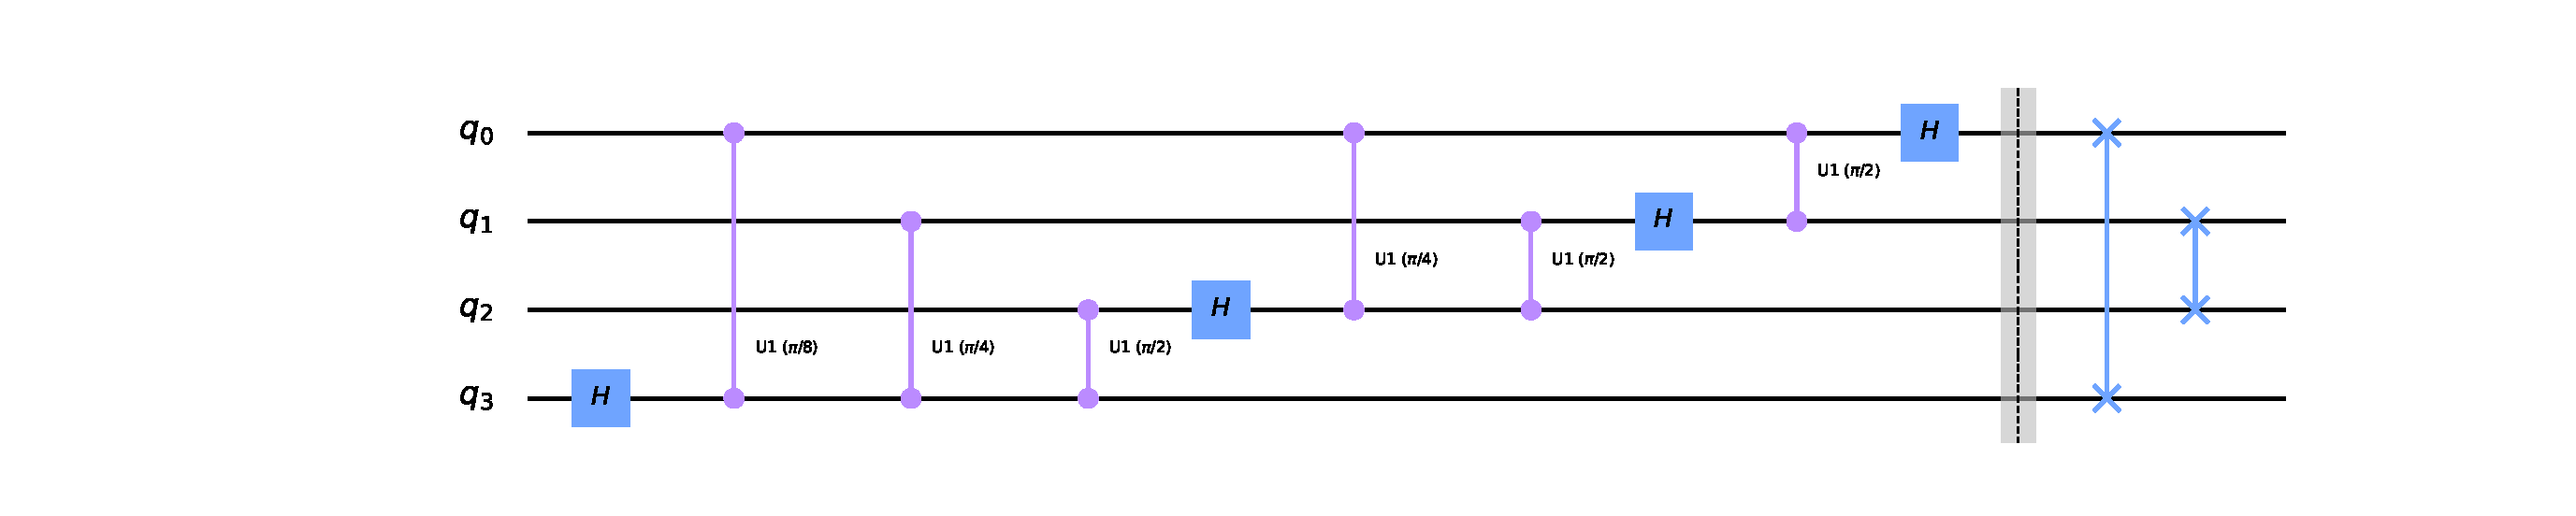
\includegraphics[width=\textwidth]{res/qft-4-qubits-circuit.pdf}
    \caption{Qiskit 4-qubit QFT circuit graph}
    \label{fig:qft-4-qubit-circuit}
\end{figure}

\paragraph{Testing}

Testing the results of the quantum Fourier transform on a simulator and a real backend.

\subsection{QFT circuit changes for error-correction}
\label{subsec:qft-circuit-error-correction}

\paragraph{Testing}
